% Plantilla para documentos LaTeX para enunciados
% Por Pedro Pablo Aste Kompen - ppaste@uc.cl
% Licencia Creative Commons BY-NC-SA 3.0
% http://creativecommons.org/licenses/by-nc-sa/3.0/

\documentclass[12pt]{article}

% Margen de 1 pulgada por lado
\usepackage{fullpage}
% Incluye gráficas
\usepackage{graphicx}
% Packages para matemáticas, por la American Mathematical Society
\usepackage{amssymb}
\usepackage{amsmath}
% Desactivar hyphenation
\usepackage[none]{hyphenat}
% Saltar entre párrafos - sin sangrías
\usepackage{parskip}
% Español y UTF-8
\usepackage[spanish]{babel}
\usepackage[utf8]{inputenc}
% Links en el documento
\usepackage{hyperref}
\usepackage{fancyhdr}
% Enumeracion con letras
\usepackage{enumitem}
\setlength{\headheight}{15.2pt}
\setlength{\headsep}{5pt}
\pagestyle{fancy}

\newcommand{\N}{\mathbb{N}}
\newcommand{\Exp}[1]{\mathcal{E}_{#1}}
\newcommand{\List}[1]{\mathcal{L}_{#1}}
\newcommand{\EN}{\Exp{\N}}
\newcommand{\LN}{\List{\N}}

\newcommand{\comment}[1]{}
\newcommand{\lb}{\\~\\}
\newcommand{\eop}{_{\square}}
\newcommand{\hsig}{\hat{\sigma}}
\newcommand{\ra}{\rightarrow}
\newcommand{\lra}{\leftrightarrow}

% Cambiar por nombre completo + número de alumno
\newcommand{\alumno}{Gonzalo Balladares - 2262595J}
\rhead{Tarea 6 - \alumno}

\begin{document}
\thispagestyle{empty}
% Membrete
% PUC-ING-DCC-IIC1103
\begin{minipage}{2.3cm}

\includegraphics[width=2cm]{img/logo.pdf}
\vspace{0.5cm} % Altura de la corona del logo, así el texto queda alineado verticalmente con el círculo del logo.
\end{minipage}
\begin{minipage}{\linewidth}
\textsc{\raggedright \footnotesize
Pontificia Universidad Católica de Chile \\
Departamento de Ciencia de la Computación \\
IIC1253 - Matemáticas Discretas \\}
\end{minipage}


% Titulo
\begin{center}
\vspace{0.5cm}
{\huge\bf Tarea 6}\\
\vspace{0.2cm}
\today\\
\vspace{0.2cm}
\footnotesize{2º semestre 2024 - Profesores P. Bahamondes - D. Bustamante - M. Romero}\\
\vspace{0.2cm}
\footnotesize{\alumno}
\rule{\textwidth}{0.05mm}
\end{center}


\section*{Pregunta 1}

\subsection*{(a)}

Sea $G=(V,E)$ un grafo, y sea $G_c=(V_c,E_c)$ el mayor clique de $G$.

Por definición se cumple que $G_c \subseteq G$.

Además se giene que $\omega(G) = |V_c|$, tenemos los siguentes casos:

\begin{enumerate}
    \item $G = G_c$:
        En este caso se tiene que $G$ es un clique, con lo que es el mayor clique de sí mismo. 
        Con lo anterior se tiene que $\omega(G) = |V_c| = |V|$.
        Luego, al ser $G$ un clique, se tentrá que $\chi(G) = |V|$, con lo que se cumple que $\omega(G) = \chi(G)$.
    \item $G_c \subseteq G \wedge G_c \neq G$:
        En este caso se tiene que existe un clique $G_c$ tal que es el mayor clique de $G$,
        el cual no es un clique en sí mismo, con lo que se tiene que $|V_c| < |V|$.
        Luego, como $G_c$ es un clique de $G$, se tiene que el mínimo coloreo posible no puede ser menor a
        la cantidad de vértices del clique, con lo que $\omega(G) \leq \chi(G)$.
    \item $G_c = \emptyset$:
        En este caso se tiene que el grafo $G$ no contiene ningún clique, con lo se $\omega(G) = |V_c| = 0$.
        Luego, al $G$ no contener ningún clique, se cumple trivialmente que $\chi(G) \leq \chi(G)$.
\end{enumerate}


\newpage
\subsection*{(b)}

Sea $G$ un ciclo de largo $n=2k+1 \geq 3$, se tiene que el tamaño máximo de $G$ es $\omega(G) = 2$,
ya que el ciclo contiene dos vértices adyacentes que forman un clique de tamaño 2. Por otra parte, 
se tiene  que el menor coloreo para $G$ es $\chi(G) = 3$, puesto que con 2 colores se estaría coloreando
dos vértices adyacentes con el mismo color, mientras que si se coloreara con 4 se tendría redundancia de colores.

Lo anterior es un caso donde se cumple que $\omega(G) < \chi(G)$, que se ilustra en la siguiente imagen para $n=5$:
\begin{center}
    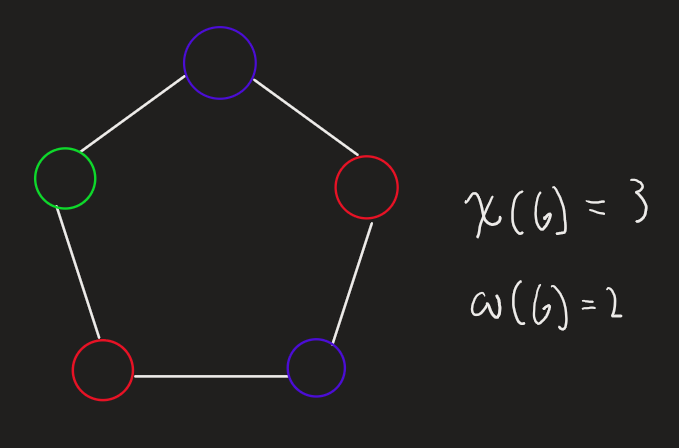
\includegraphics[width=10cm]{img/G2k1.png}
\end{center}

\subsection*{(c)}

Sea $G=(V,E)$ un grafo de tamaño $n$ y sean $V_1, V_2, \ldots, V_{\chi(G)}$ conjuntos independientes de $G$ tales que $\bigcup_{i=1}^{k} V_i = V$.
Se tendrán tantos conjuntos independientes como colores en un coloreo óptimo $\chi(G)$, siendo cada color un conjunto independiente.

Por definición tendremos que $|V_i| \leq \alpha(G) \quad \forall i \in \{1, 2, \ldots, \chi(G)\}$.
Luego, tenemos que $\sum_{i=1}^{\chi(G)} |V_i| = n$, pues si juntamos todos los vértices presentes en cada conjunto dindependiente
tendremos la totalidad de vértices del grafo.

Con lo anterior, podemos acotar superiormente la cantidad de nodos de $G$ como la sumatoria de los tamaños de los conjuntos independientes,
con el caso donde todos los conjuntos independientes son de igual tamaño, donde tendríamos $\chi(G)$ conjuntos independientes de tamaño $\alpha(G)$.

\begin{equation*}
    n = \sum_{i=1}^{\chi(G)} |V_i| \leq \chi(G) \cdot \alpha(G)
\end{equation*}

Con lo anterior se demuestra que $n \leq \chi(G) \cdot \alpha(G)$ para todo grafo $G$ con $n$ vértices.

\newpage

\section*{Pregunta 2}

\subsection*{(a)}

Sea $T=(V,E)$ un árbol con $n$ vértices.

PD: Para todo árbol con al menos 2 vértices tiene al menos 2 vértices de grado 1.

La demostración se hará mediante inducción fuerte:

\textbf{CB:} $n=2$

En este caso se tiene que el árbol $T$ tiene 2 vértices, con lo que se cumple trivialmente que al menos 2 vértices tienen grado 1.

\textbf{HI:} Todo árbol con $n$ vértices, con $n \geq 2$, tiene al menos 2 vértices de grado 1.

\textbf{TI:} Sea $T$ un árbol con $n+1$ vértices.
Sea $v$ un vértice de grado 1 en $T$, se tiene que al remover $v$ se obtiene un árbol $T'$ con $n$ vértices.
Por hipótesis se tiene que $T'$ tiene al menos 2 vértices de grado 1, con lo que se tiene que $T$ tiene al menos 2 vértices de grado 1.

Con lo anterior se concluye que para todo árbol con al menos 2 vértices tiene al menos 2 vértices de grado 1.

\newpage
\subsection*{(b)}

Se demostrará mediante inducción sobre el número de vértices del torneo.

PD: Todo torneo tiene un camino hamiltoniano.

Sea $G=(V,E)$ un torneo con $n$ vértices.

\textbf{CB:} $n=1$

En este caso se tiene que el torneo $G$ tiene un solo vértice, con lo que se cumple trivialmente que tiene un camino hamiltoniano.

\textbf{HI:} Se asume que para todo torneo con $n$ vértices, existe un camino hamiltoniano.

\textbf{TI:} Sea $G$ un torneo con $n+1$ vértices.

Sea $v$ un vértice cualquiera de $G$, se tiene que al remover $v$ se obtiene un torneo $G'$ con $n$ vértices.
Por hipótesis se tiene que $G'$ tiene un camino hamiltoniano, el cual estará compuesto por los vértices $V = \{v_1, v_2, \ldots, v_n\}$.

Si se agrega el vértice $v$ al camino hamiltoniano de $G'$, se tiene queire demostrar que el nuevo torneo tiene camino hamiltoniano,
para lo cual tenemos 3 casos:

\begin{enumerate}
    \item $v$ es el vértice inicial del camino hamiltoniano:
        En este caso se tiene que $v$ tiene una arista en dirección $(v, v_n)$, con lo que se tiene un camino hamiltoniano.
    
    \item $v$ es el vértice final del camino hamiltoniano:
        De manera similar, en este caso se tiene que $v$ tiene una arista en dirección $(v_1, v)$, con lo que se tiene un camino hamiltoniano.

    \item $v$ está en medio del camino hamiltoniano:
        En este caso, por hipótesis se tendrá que existe al menos un vértice $v_i$ tal que $v$ tiene una arista en dirección $(v_i, v)$ y otra en dirección $(v, v_{i+1})$,
        con lo que se tiene un camino hamiltoniano que irá en dirección
        $v_1 \ra v_2 \ra \ldots \ra v_i \ra v \ra v_{i+1} \ra \ldots \ra v_n$.
\end{enumerate}

Finalmente, se concluye que para todo torneo existe un camino hamiltoniano.

\end{document}
